\chapter{Concurrent Programming and Verification}
In chapter \ref{chap:verlixir}, we will introduce the Verlixir tool. Verlixir involves the parsing of Elixir programs, which are translated into a formal model. This model is written in Process Meta Language (Promela). This chapter will introduce both Elixir and Promela. We will go through the core concepts and syntactic elements that Verlixir relies upon to provide a verification-aware Elixir. 
\section{Promela} \label{sec:promela}
Promela is the verification modelling language used by the Spin model checker, to specify concurrent processes modelling distributed systems \cite{spin}. This section will discuss some of the core features that allow systems to be modelled and verified with Spin. This section aims to give an overview of the syntax and control of Promela, so any specifications in later sections or the code artifact can be read.
\subsection{Types and Variables}
Promela is statically typed. Variables can be declared once within the current scope and then re-assigned throughout. Variables can be declared locally within the context of a process, or in the global scope, where memory is shared. The types available in Promela, and assignment to variables of these types if similar to many imperative programming languages. Promela supports the types bit, bool, byte, pid, short, int and unsigned. Variable declaration and assignment then naturally follows.
\[
\begin{aligned}
\text{int a} = 2;
\end{aligned}
\]
\subsection{Control Flow}
Promela supports some basic control flow concepts. Firstly, the \texttt{skip} expression can be used with no effect when executed, other than possibly changing the control of an executing process. The selection construct \texttt{if} can be used to evaluate expressions and execute sequences based on the evaluation of these expressions. The syntax of an if statement is unique in comparison to a typical programming language.
\[
\begin{aligned}
& \text{if} \\
& :: \text{exp\_1 ->} \dots \\
& :: \text{exp\_2 ->} \dots \\
& \text{fi} \\
\end{aligned}    
\]
Repetition can be achieved either through the \texttt{do} construct, through the use of labels or with \texttt{for} loops.
\subsection{Processes}
An imperative component of understanding the power of the Spin model checker is understanding how processes can run concurrently. Every Promela model requires an initial process that is spawned in the initial system state and determines the control of the program from the initial state. The \texttt{init} keyword is reserved for this purpose. Other processes can be defined using the \texttt{proctype} keyword and then spawned with \texttt{run}. Each process is assigned a process id (pid) which can be accessed within the context of a process using globally defined read-only variable \texttt{\_pid}. We can now define two processes, a process active in the initial state and a second process that is spawned.
\begin{lstlisting}[language=promela, xleftmargin=.3\linewidth, caption={Defining and spawning processes in Promela}., label={fig:promela_processes}]
    proctype SomeProcess(int a) {
        printf("Do something with %d\n", a);
    }
    
    init {
        int p1;
        p1 = run SomeProcess(10);

        printf("Init process spawned at %d\n", _pid);
        printf("Process 1 spawned at %d\n", p1);
    }
\end{lstlisting}
Multiple processes can be declared to run in the initial state by marking them as \texttt{active} processes. Processes run independently of one another, so a parent process terminating will not necessarily result in the termination of a child. Spin sets a limit of 255 concurrently executing processes. Multiple processes can be spawned in a single transition by using the \texttt{atomic} construct, which will ensure that no spawning process is scheduled until all atomic processes have been scheduled. Similarly to atomicity, \texttt{d\_step} can be used to enforce multiple statements are treated as a single indivisible step. Unlike \texttt{atomic}, \texttt{d\_step} cannot block or jump.
\subsection{Channels}
The final concept to briefly discuss is the asynchronous communication primitive, channels. Recall Hoare's definition of channels \ref{csp_section}, defining a channel $c$ that can input and output values. Promela echos this definition, allowing channels to be specified using the predefined data type \texttt{chan}. To correctly specify communication, we often need to allow messages of multiple types to be written to channels, for this purpose Promela introduces \texttt{mtype} that allows for the introduction of symbolic names for constant values.
\[
\text{mtype = \{ BROADCAST \};}
\]
Now, we can define a channel that expects a message to contain multiple fields and is bound to contain a maximum of 10 messages at any time.
\[
\text{chan global\_broadcast = [10] of \{ mtype, int \};}
\]
We now input messages to the channel using the (!) operator.
\[
\text{global\_broadcast ! BROADCAST, 1;}
\]
Similarly, we read messages from the channel in a first-in, first-out (FIFO) order.
\[
\begin{aligned}
& \text{int x;} \\
& \text{global\_broadcast ? BROADCAST, x;}
\end{aligned}
\]
Where the variable $x$ stores the resulting \texttt{int} assuming the first message in the channel is of type \texttt{BROADCAST}.
\subsection{Limitations}
Promela is a powerful language for modelling concurrent systems, but it has limitations for capturing the full complexity of a real-world system. In general, hand-translations of a system into Promela can avoid some of these limitations with careful design. However, we are approaching this limits from an Elixir perspective, where features of Elixir may not be easily translated into Promela.
\begin{itemize}
    \item \textbf{Compute}: Promela is not designed to model complex computations. It does not support floating-point arithmetic, so we are limited to working with integers.
    \item \textbf{Memory}: Promela does not support dynamic memory allocation. This means we cannot model systems that require dynamic memory allocation, for example, linked lists.
    \item \textbf{Functions}: Promela does not support functions. It has no notion of a function call or return. By extension, Promela does not support recursion.
    \item \textbf{Randomness}: a Spin execution may not be deterministic, but it cannot model true randomness.
    \item \textbf{Probability}: there is no mechanism for modelling probabilistic behaviour, all correctness claims are checked unconditionally.
    \item \textbf{Time}: there is no notion of a system block, or related time properties in Promela. This means we cannot model sleeping threads.
\end{itemize}
\subsection{Summary}
This basic introduction to the syntax of the Promela modelling language aims to make the reader familiar with the syntax and control involved in writing Promela specifications. It is not an exhaustive guide but should form a basis for understanding specifications present in a later section or the code artifact.

\section{Elixir}
Elixir is a dynamic, functional language for building scalable and maintainable applications \cite{elixir}. Elixir programs run on the BEAM virtual machine \cite{beam}, which is also used to run the Erlang programming language \cite{erlang}. Elixir was designed by José Valim and first released in 2012. Elixir is built on top of Erlang and hence inherits many of the abstractions designed for building distributed systems. This section aims to give a brief overview of Elixir, it is not a complete guide but rather aims to give non-Elixir programmers a basic understanding of the language.
\\ \\
BEAM is a virtual machine that executes user programs in the Erlang Runtime System (ERTS). BEAM is a register machine where all instructions operate on named registers containing Erlang terms such as integers or tuples.
\\ \\
Elixir has begun to see use in industry, in particular in domains such as telecoms and instant messaging. The Phoenix Framework \cite{phoenix} is a framework for building interactive web applications natively in Elixir that can take advantage of Elixir's multi-processing and fault tolerance to build scalable web applications. The audio and video communication application Discord \cite{discord} uses Elixir to manage its 11 million concurrent users and the Financial Times \cite{ft} have begun migrating from Java to Elixir to enjoy the much smaller memory usage by comparison.
\\ \\
Elixir supports multi-processing in two key ways: nodes and processes. Each node is an instance of BEAM (a single operating system process), when an Elixir program is executed, a new instance of BEAM is instantiated for it to run on. In contrast, an Elixir process is not an operating system process. An Elixir process is lightweight in terms of memory and CPU usage (even in comparison to threads that many other programming languages favour). Elixir processes can run concurrently with one another and are completely isolated from one another. Elixir processes communicate via message passing.
\begin{lstlisting}[language=Elixir, xleftmargin=.2\linewidth, caption={An example of spawn/1 and spawn/4 in Elixir for spawning a new lightweight process and a new Elixir node}]
    # Spawn a new process
    spawn(fn -> 1 + 2 end)

    # Create a new BEAM instance
    Node.spawn(:"node1@localhost", MyModule, :start, [])
\end{lstlisting}
\subsection{Shared Memory and Message Passing}
Two key concepts in inter-process communication (IPC) are shared memory models and message-passing models. They are two techniques used to allow processes to send signals or share data between each other. In a shared memory model, a shared memory region is established in which multiple processes can read and write. Figure \ref{fig:shared_memory} shows a basic example of two processes that write to a shared in-memory array. Due to how often we see shared memory used in large-scale distributed systems, much work has been done in the verification of these systems using shared memory models. For example, Jon Mediero Iturrioz used Dafny \cite{dafny} to prove the correctness of concurrent programs that implement shared memory \cite{shared_memory_verification}. 
\begin{figure}[h]
    \centering
    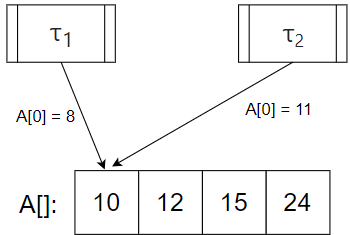
\includegraphics[width=0.4\textwidth]{images/shared_memory.png}
    \caption{An example of two processes writing to a shared in-memory array}
    \label{fig:shared_memory}
\end{figure}
\\ \\
Elixir instead uses a message-passing model for IPC. More specifically, Elixir uses an actor-based model, where each process (actor) has its state and a message box to receive messages from other actors. Actors are responsible for sending a finite number of messages to other actors, spawning new actors and changing their behaviour based on the handling of messages received in the mailbox. Figure \ref{fig:actor_model} shows an example of how actors behave. The mailbox is not necessarily first in, first out (FIFO) but often implementations tend to be.
\begin{figure}[H]
    \centering
    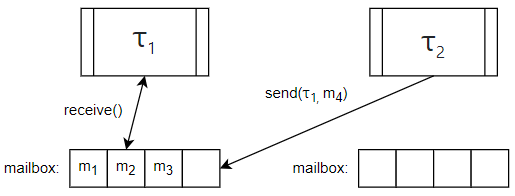
\includegraphics[width=0.6\textwidth]{images/actor_model.png}
    \caption{An example of actors sending and receiving messages under the actor model}
    \label{fig:actor_model}
\end{figure}
In Elixir, a receive statement is used to read messages in the mailbox. The receive block looks through the mailbox for a message that matches a given pattern, if no messages match a given pattern, the process will block until one does.
\begin{lstlisting}[language=Elixir, xleftmargin=.4\linewidth, caption={An example of spawn/1 and spawn/4 in Elixir for spawning a new lightweight process and a new Elixir node}]
    # Example send in Elixir
    send self(), {:hello, "world"}

    # Example receive block in Elixir
    receive do
        {:hello, msg} -> IO.puts msg
    end
\end{lstlisting}
\subsection{Verifiable Feature Set} \label{sec:verifiable_feature_set}
In chapter \ref{chap:verlixir}, we will introduce Verlixir. Verlixir is designed to support a reduced set of core Elixir constructs. We will introduce these constructs here to give an overview of what the tool is capable of supporting.
\\ \\
Everything in Elixir is an expression. This means that every piece of code returns a value. For example, an $if$ statement will return a value dependent on the branch taken. This means that any expression can be matched on, using Elixir's match (=) operator. We can use pattern matching to match on the shape of an expression's evaluation. The set of expressions supported by Verlixir are:
\begin{itemize}
    \item \textbf{Values}: any value of a basic, primitive type such as integers and booleans. Elixir also has a concept of $atoms$. An atom is identified by a preceding colon (:), and is followed by letters, digits, `\_', `@' or a string.
    \item \textbf{Variables}: Elixir is dynamically, strongly typed. Variables are bound to using the match operator. Variable names start with lowercase letters. The `\_' character can be used to match an expression of any shape.
    \item \textbf{Data structures}: structures such as lists and tuples are treated as values. Lists are dynamic, whereas tuples are fixed in size. Lists are written as [1, 2, 3] and tuples are written as \{1, 2, 3\}. We can match on the shape of these data structures using pattern matching.
    \item \textbf{Pattern matching}: pattern matching can be used to match on the shape of an expression. In the context of a conditional guard, values can be used to evaluate the shape of an expression, where as variables can be used to bind to the value of an expression. For example, the pattern ${:ok, value}$, can be used to assign to the variable $value$ if the expression is a tuple shape, with an atom $ok$ as the first element.
    \item \textbf{Functions}: functions are defined using the $def$ keyword. Functions can group multiple sequentially executable expressions. Any function can be called or spawned as a new process or node.
    \item \textbf{Modules}: functions are grouped into modules.
    \item \textbf{Message passing}: Elixir's actor model supports message passing. Messages are sent and received between actors and their mailboxes.
    \item \textbf{Control flow structures}: Elixir supports many control flow expressions. For example, $if$, $case$, $unless$ and $for$. All of these introduce a new scope. They are expressions and can be matched on.
\end{itemize}
\subsection{Summary}
In this chapter, we learned about Elixir, the programming language built on top of Erlang and we explored some basic approaches to designing concurrent systems with it. The next    section will explore how these core tools can be used in tandem to provide developers guarantees over large-scale, distributed Elixir-based systems.